% TEX compiler = luatex
% copyright arturo salinas-aguayo 2025
\documentclass[12pt]{article}

\usepackage{graphicx}
\usepackage{subcaption}
\usepackage{amsmath}
\usepackage{array}
\usepackage{amsfonts}
\usepackage{fancyhdr}
\usepackage{geometry}
\usepackage{circuitikz}
\usepackage{subfigure}
\usepackage{caption}
\usepackage{karnaugh-map}
\usepackage{bm}
\usepackage{float}

\geometry{letterpaper, margin=1in}
\graphicspath{ {../../images/} }

% Header and Footer
\pagestyle{fancy}
\fancyhf{}
\fancyhead[L]{ECE 2001 - Lab 05: First-Order Circuits}
\fancyhead[R]{\thepage}
\setlength{\headheight}{15pt}

\author{Arturo Salinas-Aguayo}
\title{Lab 05: First-Order Circuits}

% theorem set
\newtheorem{example}{Example}
% Example block environment
\newenvironment{examp}
{\vspace{0.5cm}
 \hrule
\vspace{0.5cm}
\begin{example}}
{\hrule
\vspace{0.5cm}
\end{example}}

\begin{document}
\newcommand{\closure}[2][3]{%
	{}\mkern#1mu\overline{\mkern-#1mu#2}}
\newcommand\ncoverline[1]{\mkern1mu\overline{\mkern-1mu#1\mkern-1mu}\mkern1mu}
% Title Page
\begin{titlepage}
	\centering
	\vspace*{3cm}
	\huge\textbf{Lab 05: First-Order Circuits}\\
	
	\vspace{5cm}
	\Large\textbf{Arturo Salinas-Aguayo}\\
	\normalsize
	ECE 2001 Electrical Circuits\\
	Dr. David J. Giblin, Section 331.660.701.810-1253\\
	Mechanical Engineering Department
	\vfill
	
\includegraphics[scale=0.1]{uconnlogo}\\
	College of Engineering, University of Connecticut\\
	\scriptsize{Coded in \LaTeX}
	\vspace*{1cm}
\end{titlepage}
\tableofcontents
\newpage
\section{Abstract}
The course has so far introduced a few analog components such as resistors,
LEDs, Operational Amplifiers, microphones, and speakers, however the use of
other passive elements such as capacitors and inductors has been somewhat
limited to filter out noise from the sound mixer design project. This week's
experimental work creates the next leap by introducing the analysis of the
capacitor and inductor which lead to first-order linear differential equations.
By studying these and their use in circuits, although quite limited for DC
applications, the ability to understand the response of these components allows
for the further study of circuits involving both capacitive and inductive
components. 
\newpage
\section{Introduction}
First-Order circuits are characterized by a first-order linear differential
equation. This may seem a bit overwhelming at first, but a common theme in the
experimental work is to build intuition with the analysis of these circuits
and simplify the analysis greatly by being able to calculate the Thevenin or
Norton equivalent circuit and fitting an algebraic equation to match the
behavior of the inductive or capacitive component.

Up until now, all components analyzed have been static components for the most
part. Node voltages stay the same once solved and branch currents also stay
constant. The inclusion of the inductor and capacitor moves away from this and
introduces a \textit{time} based component to the analysis where depending on
the value of the inductor or capacitor, a circuits response will vary in
\textit{time constants}.

The Node Voltage Method and the Mesh Current Method still apply to these
circuits and can always be relied upon in a pinch in case the analyzer becomes
befuddled or confused about how the branch response affects the rest of the
circuit, however knowing the general form and behavior of these circuits allows
for much of the more complicated math to be bypassed completely.
\section{Theory}
\subsection{RC Circuits}
A \textit{Resistive Capacitive}, or RC circuit is simply one which contains a
resistive element and a capacitive element. One is shown in Figure
\ref{fig:theory1}.
\begin{figure}[H]
	\centering
	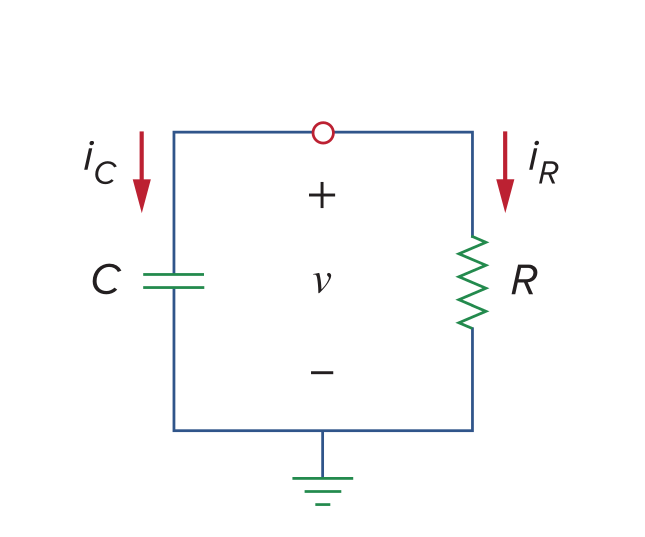
\includegraphics[width=5cm]{e5_th1}
	\caption{An RC Circuit}
	\label{fig:theory1}
\end{figure}
A capacitor is said to block DC voltage at steady state, that is, when there is
no change or step response from the sources, the capacitor resembles an open
circuit. However, when a sudden change or step response from the throwing of a
switch or the application of a source, the capacitor contributes to the response
of the circuit. 

The natural response of the capacitor is such that its voltage (remember that
voltage corresponds with a force in the physical world), cannot change suddenly,
however the current flow of a capacitor will have discontinuities. Working from
the circuit in Figure \ref{fig:theory1}, KCL at the top node produces:
\[
	i_C + i_R = 0
\]
Where $i_C = C \frac{dv}{dt}$ and $i_R = \frac{v}{R}$.
Eventually, once the differential equation is solved by separation of variables,
the following exponential equation is obtained:
\[
	v(t) = V_0e^{-t/RC}
\]
Notice that the power which the exponential is raised to depends on two factors.
The product of $RC$ and a new variable, $t$ which stands for time. $RC$ is the
product of these two values in which resistance is in ohms and capacitance is in
Farads. The product of these two values produces a unit of \textit{seconds}.

Therefore, it is commonly notated as
\[
	\tau = RC
\]
The dynamic nature of the circuit dies down after about 5 time constants where
the circuit is, for all intensive purposes, considered to be at steady state
again and the capacitor again appears like an open circuit at its leads.

When a stepped input is added as alluded to earlier, the equation becomes:
\[
	v(t) = v(\infty) + [v(0) - v(\infty)]e^{-t/\tau}
\]
Where $v(0)$ is the initial voltage felt at the ``Open" of the capacitor, and
$v(\infty)$ is the final voltage felt at the ``Open" of the capacitor. $\tau$ is
the Thevenin resistance of the final circuit and the value of the capacitor. 

\subsubsection{The Technique}
The best method to analyze RC circuits is again by utilizing some intuition
and following a simple procedure to obtain initial, transient, and final
responses.
\begin{enumerate}
	\item Find Thevenin Equivalence at initial values.
	\item Find Thevenin Equivalence at final values.
	\item Analyze and plug in constants to obtain transient response equations
\end{enumerate}
That's it. No need to muddle about with differential equations or anything of
the sort. A similar method exists for RL circuits.

\subsection{RL Circuits}
A \textit{Resistive Inductive}, or RL circuit is one which contains a resistive
element and an inductive element. One such configuration is shown in Figure
\ref{fig:theory2}.

\begin{figure}[H]
	\centering
	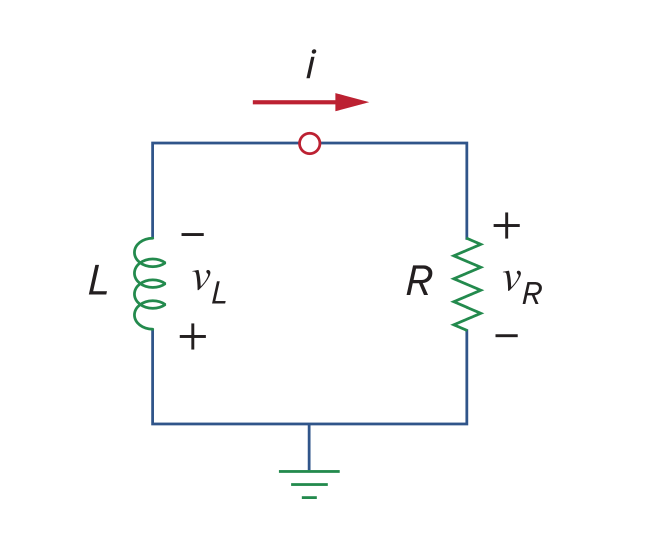
\includegraphics[width=5cm]{e5_th2}
	\caption{An RL Circuit}
	\label{fig:theory2}
\end{figure}

An inductor, in contrast to a capacitor, is said to block changes in current.
At steady state (i.e., after all transients have died out), an inductor behaves
like a short circuit, offering no resistance to current flow. However, during
transients—like when a switch is thrown or a source is applied—the inductor
resists changes in current, and this gives rise to the circuit's time-dependent
behavior.

Recall that voltage across an inductor is defined as:
\[
	v_L = L \frac{di}{dt}
\]
While the voltage across the resistor is:
\[
	v_R = iR
\]

Applying KVL around the loop of Figure \ref{fig:theory2} gives:
\[
	v_L + v_R = 0
	\Rightarrow L \frac{di}{dt} + iR = 0
\]

Solving the differential equation yields an exponential decay of current:
\[
	i(t) = I_0 e^{-t/RC}
\]
But since this is an RL circuit, the time constant is instead:
\[
	\tau = \frac{L}{R}
\]

As before, this $\tau$ has units of seconds and represents the characteristic
time it takes for the transient to decay significantly. After approximately
5$\tau$, the inductor's effect is negligible, and the circuit is considered to
have reached steady state.

When a stepped source is added, the current response becomes:
\[
	i(t) = i(\infty) + [i(0) - i(\infty)]e^{-t/\tau}
\]
Where $i(0)$ is the initial current through the inductor (which cannot change
suddenly), and $i(\infty)$ is the final current the inductor allows at
steady-state. $\tau = \frac{L}{R}$, with $L$ in Henries and $R$ in Ohms.

\subsubsection{The Technique}
Just like the RC case, RL circuits are analyzed by identifying initial,
transient, and final behavior:
\begin{enumerate}
	\item Find the Norton equivalent circuit seen by the inductor initially.
	\item Find the Norton equivalent circuit seen by the inductor at final
	      conditions.
	\item Analyze and plug in constants to obtain transient response
	      equations.
\end{enumerate}

\subsection{The Shape of the Response}
Knowing the fact that these two differential equations refer to an exponential
equation is quite a strong observation. This allows for only two options
graphically depending on the circuit. Either the voltage is building
exponentially or decreasing exponentially in the same shape always—or the
current is.

This exponential shape is always the same: it either rises from an initial value
toward a final value asymptotically, or it decays from some initial value down
toward zero. The only difference lies in what the initial and final values are,
and whether it’s voltage or current we’re examining. Regardless, the time
constant $\tau$ controls how "fast" or "slow" this curve progresses.

For a rising exponential (build-up), such as when a capacitor charges or current
ramps up in an inductor:
\[
	y(t) = y(\infty) \left(1 - e^{-t/\tau}\right)
\]

For a falling exponential (decay), such as when a capacitor discharges or an
inductor’s current dies out:
\[
	y(t) = y(0) e^{-t/\tau}
\]

These expressions describe the same curve flipped around—either rising or
falling depending on the physical setup. Figures \ref{fig:rising_exp} and
\ref{fig:falling_exp} show both cases.

\begin{figure}[H]
	\centering
	\begin{subfigure}[b]{0.45\linewidth}
		\centering
		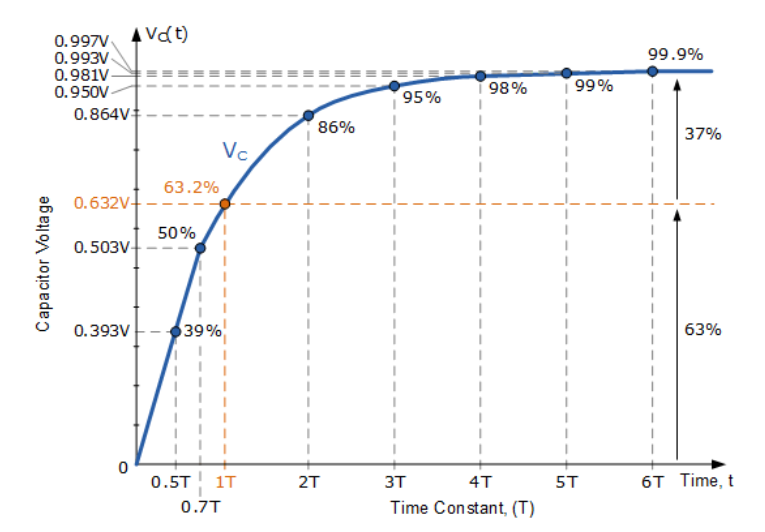
\includegraphics[width=\linewidth]{rising_exp}
		\caption{Rising Exponential Response}
		\label{fig:rising_exp}
	\end{subfigure}
	\hfill
	\begin{subfigure}[b]{0.45\linewidth}
		\centering
		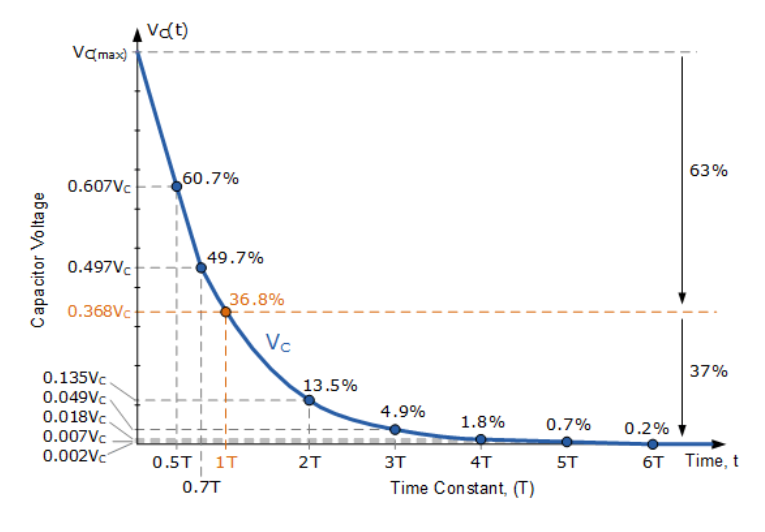
\includegraphics[width=\linewidth]{falling_exp.png}
		\caption{Falling Exponential Response}
		\label{fig:falling_exp}
	\end{subfigure}
	\caption{Exponential response shapes in first-order circuits.}
	\label{fig:exp_shapes}
\end{figure}

After one time constant $\tau$, the curve has reached about 63\% of the way to
its final value. After about 5$\tau$, it’s considered close enough to steady
state that the transient is effectively over.

This universal shape simplifies analysis and allows for more of an intuition of
how the circuit will behave.


\section{Experimental Procedures}

\subsection{Circuit One: Charging (Growth)}
The first experimental setup focused on observing the charging behavior of a capacitor in a high-impedance RC circuit. With no initial voltage across the capacitor and a DC supply of $10\,\mathrm{V}$ applied at $t = 0$, the capacitor begins charging through a $10\,\mathrm{M}\Omega$ resistor.

\begin{figure}[H]
	\centering
	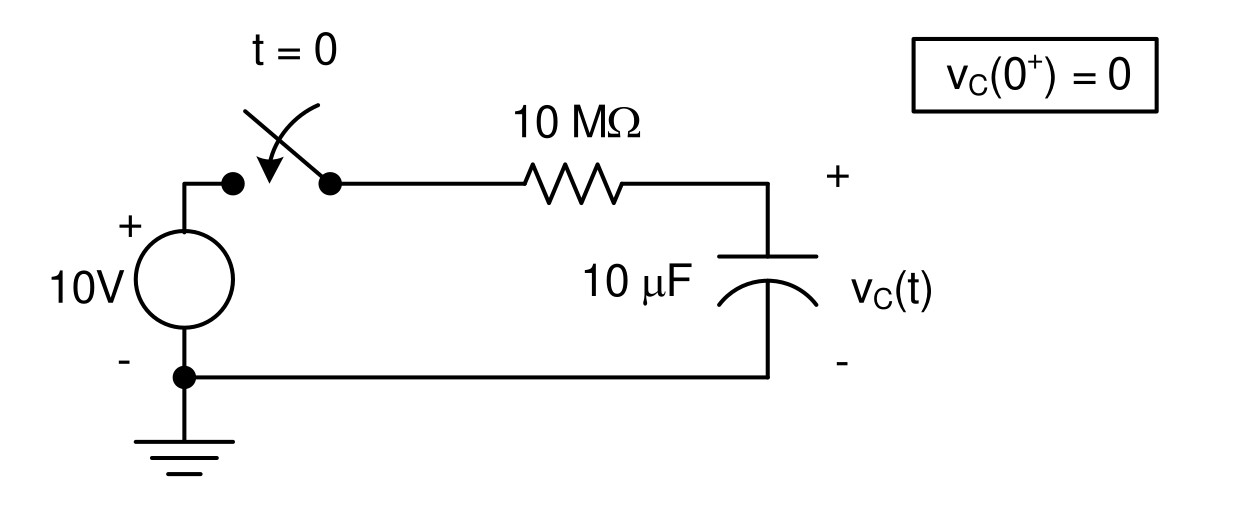
\includegraphics[width=\textwidth]{e5_1}
	\caption{RC Circuit Undergoing Charging (Virgin Configuration)}
	\label{fig:circuit1}
\end{figure}

The component values were:
\[
	V_0 = 0\,\mathrm{V}, \quad R = 10\,\mathrm{M}\Omega, \quad C = 10\,\mu\mathrm{F}, \quad V_f = 10\,\mathrm{V}
\]
\[
	\tau = RC = 10\,\mathrm{M}\Omega \cdot 10\,\mu\mathrm{F} = 100\,\mathrm{s}
\]

This relatively large time constant results in a slow rise in voltage across the capacitor. The expected transient response is given by:
\[
	v_C(t) = 10 - 10e^{-t/100}
\]

\begin{figure}[H]
	\centering
	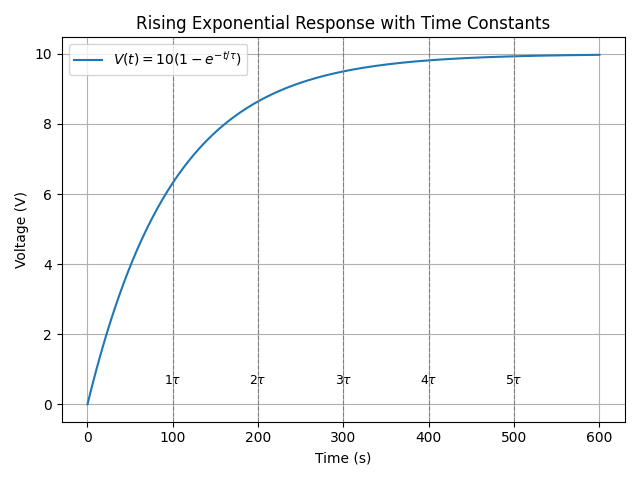
\includegraphics[width=10cm]{05_exp1}
	\caption{Expected Charging Curve for Circuit One}
	\label{fig:circuitonegraph}
\end{figure}

\subsection{Circuit One: Discharging (Decay)}
The second configuration reversed the behavior: starting with the capacitor fully charged to $10\,\mathrm{V}$ and then disconnected from the source, the voltage was allowed to decay through the same $10\,\mathrm{M}\Omega$ resistor.

\begin{figure}[H]
	\centering
	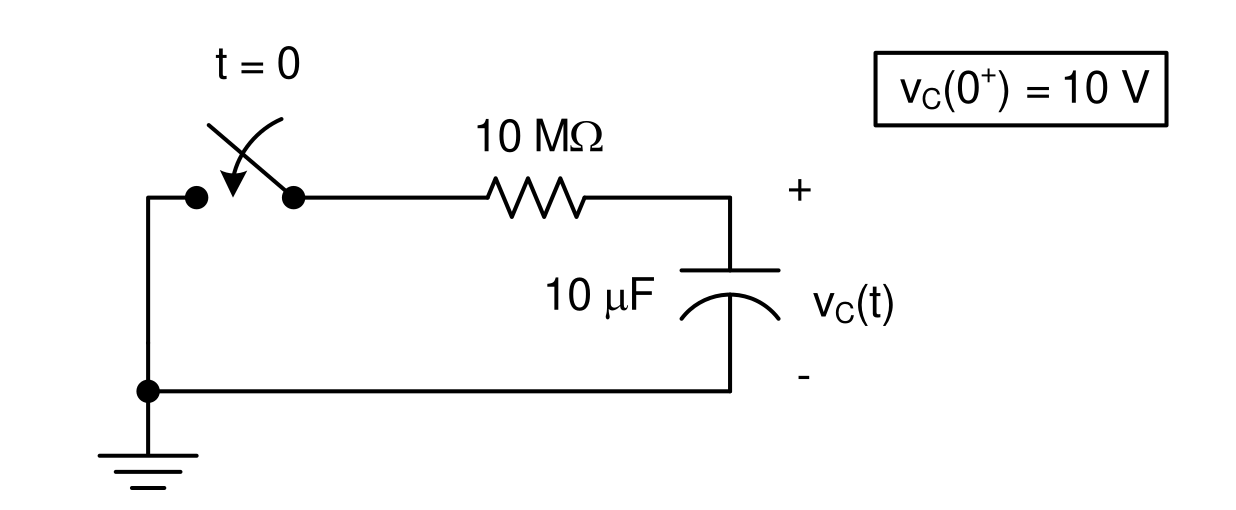
\includegraphics[width=14cm]{e5_2}
	\caption{RC Circuit Undergoing Discharge (Excited Configuration)}
\end{figure}

The parameters remained the same:
\[
	V_0 = 10\,\mathrm{V}, \quad R = 10\,\mathrm{M}\Omega, \quad C = 10\,\mu\mathrm{F}, \quad V_f = 0\,\mathrm{V}
\]
\[
	\tau = RC = 10\,\mathrm{M}\Omega \cdot 10\,\mu\mathrm{F} = 100\,\mathrm{s}
\]

The expected voltage decay follows the form:
\[
	v_C(t) = 10\,e^{-t/100}
\]

\begin{figure}[H]
	\centering
	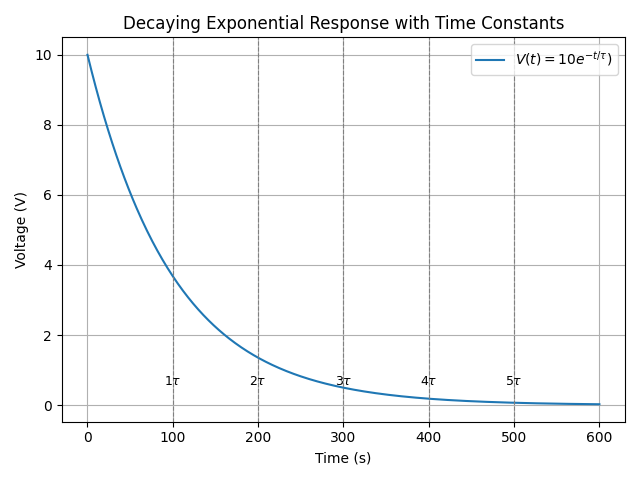
\includegraphics[width=10cm]{05_exp2}
	\caption{Expected Discharging Curve for Circuit One}
	\label{fig:circuitonegraph2}
\end{figure}

\subsection{Circuit Three: RC with Square Wave Input}
Circuit Three introduced a periodic square wave input instead of a static DC source. The capacitor alternately charges and discharges in response to the high and low states of the wave, creating a periodic exponential waveform across its terminals.

\begin{figure}[H]
	\centering
	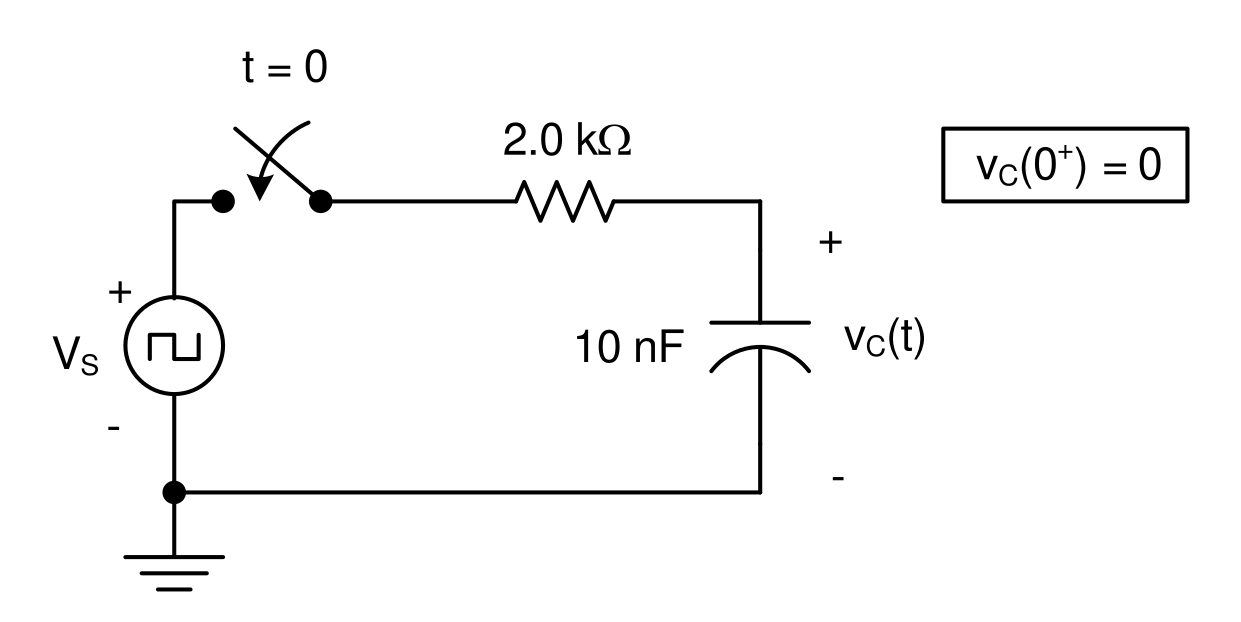
\includegraphics[width=14cm]{e5_3}
	\caption{RC Circuit with Square Wave Input}
\end{figure}

\[
	R = 2.0\,\mathrm{k}\Omega, \quad C = 10\,\mathrm{nF}, \quad V_c(0^+) = 0\,\mathrm{V}
\]
\[
	\tau = RC = 2.0\,\mathrm{k}\Omega \cdot 10\,\mathrm{nF} = 20\,\mu\mathrm{s}
\]

A square wave of $5\,\mathrm{V}$ amplitude was applied, and the period was set to:
\[
	T = 10\tau = 200\,\mu\mathrm{s}
\]

The resulting exponential voltage response for the capacitor is:
\[
	v_C(t) = 5\left(1 - e^{-t/20\mu s}\right) \quad \text{(charging)}
\]
\[
	v_C(t) = 5\,e^{-t/20\mu s} \quad \text{(discharging)}
\]

\subsection{Circuit Four: RC Circuit with Adjusted Components}
This circuit is topologically identical to Circuit Three but with different R and C values, leading to a different time constant while retaining the same input waveform structure.

\begin{figure}[H]
	\centering
	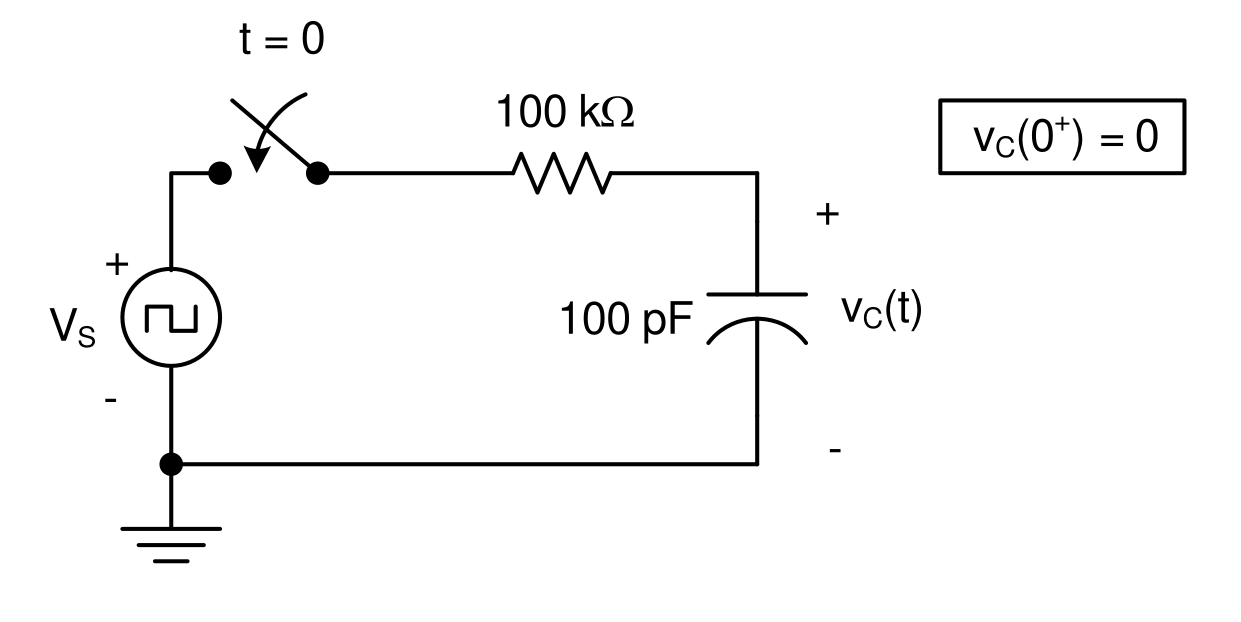
\includegraphics[width=14cm]{e5_4}
	\caption{RC Circuit with Smaller Time Constant}
	\label{circuit3}
\end{figure}

\[
	R = 100\,\mathrm{k}\Omega, \quad C = 100\,\mathrm{pF}, \quad V_c(0^+) = 0\,\mathrm{V}
\]
\[
	\tau = RC = 100\,\mathrm{k}\Omega \cdot 100\,\mathrm{pF} = 10\,\mu\mathrm{s}
\]

The square wave had an amplitude of $5\,\mathrm{V}$ and a calculated period of:
\[
	T = 10\tau = 100\,\mu\mathrm{s}
\]

Voltage response equations:
\[
	v_C(t) = 5\left(1 - e^{-t/10\mu s}\right) \quad \text{(charging)}
\]
\[
	v_C(t) = 5\,e^{-t/10\mu s} \quad \text{(discharging)}
\]

\subsection{Circuit Five: RL Response to Square Wave}
Circuit Five replaces the capacitor with an inductor and analyzes the current behavior in response to a square wave input. Due to the high voltages generated at switching transitions, the amplitude was reduced to $1\,\mathrm{V}$ for safety and clarity.

\begin{figure}[H]
	\centering
	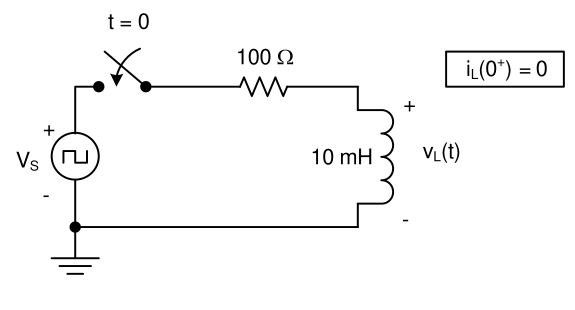
\includegraphics[width=14cm]{e5_5}
	\caption{RL Circuit with Square Wave Input}
	\label{fig:circuit5}
\end{figure}

\[
	L = 10\,\mathrm{mH}, \quad R = 100\,\Omega, \quad I_L(0^+) = 0\,\mathrm{A}
\]
\[
	\tau = \frac{L}{R} = \frac{10\,\mathrm{mH}}{100\,\Omega} = 100\,\mu\mathrm{s}
\]

The input waveform was a $1\,\mathrm{V}$ square wave with a period of:
\[
	T = 10\tau = 1.0\,\mathrm{ms}
\]

The current response is modeled by:
\[
	i_L(t) = \frac{V}{R}\left(1 - e^{-t/\tau}\right) = \frac{1}{100}\left(1 - e^{-t/100\mu s}\right) = 10\,\mathrm{mA}\left(1 - e^{-t/100\mu s}\right) \quad \text{(ramp-up)}
\]
\[
	i_L(t) = \frac{V}{R} e^{-t/\tau} = 10\,\mathrm{mA} \cdot e^{-t/100\mu s} \quad \text{(decay)}
\]

The inductor resists instantaneous current changes, leading to characteristic spikes in voltage at the moment the square wave toggles state.
\section{Results and Discussion}
\subsection{Circuit One: Charging Transient}
For the first circuit, a large time constant was calculated. This circuit
(Figure \ref{fig:circuit1}) will take a long time to charge to final voltage,
however it also serves as a reminder that measurement tools such as voltmeters
contain their own resistance which will act as loads on any given circuit. In
order to obtain clean data which represents the behavior of the capacitor,
only momentary touches of the leads to the capacitor were allowed at the
intervals shown in Table \ref{tab:charging}.

\begin{table}[H]
	\centering
	\begin{tabular}{|c|c|}
		\hline
		Time (s) & Voltage (V) \\
		\hline
		0        & 0           \\
		\hline
		20       & 1.6         \\
		\hline
		30       & 2.63        \\
		\hline
		60       & 4.00        \\
		\hline
		90       & 5.09        \\
		\hline
		120      & 5.47        \\
		\hline
		150      & 5.85        \\
		\hline
		180      & 6.15        \\
		\hline
		210      & 6.46        \\
		\hline
		240      & 6.70        \\
		\hline
		270      & 6.90        \\
		\hline
		300      & 7.10        \\
		\hline
		330      & 7.27        \\
		\hline
		360      & 7.40        \\
		\hline
		390      & 7.52        \\
		\hline
	\end{tabular}
	\caption{Measured Data for Charging Capacitor}
	\label{tab:charging}
\end{table}

The behavior of the voltage charging event was exactly as expected well within
tolerances. Due to the inherent resistance of the measurement tool, the final
capacitor voltage was a little bit lower, however for experimental purposes,
this still confirmed the time constant and behavioral characteristics.

Without the multimeter attached to the terminals, a voltage of $10\,\mathrm{V}$
equal to the supply voltage provided by the dedicated power supply was correctly
identified later, after allowing the multimeter to remain disconnected during the
charge period.

\subsubsection{Time Constant Analysis.}

From the measured data, the voltage rose toward a final value of approximately
$7.52\,\mathrm{V}$. The theoretical final value was $10\,\mathrm{V}$, but the
presence of the voltmeter's input resistance resulted in a reduced effective
final voltage.

To determine the experimental time constant, we note that at $t = \tau$, the
voltage should reach approximately $63\%$ of its final value:
\[
	V_f \approx 7.52\,\mathrm{V}, \quad V_{63\%} = 0.63 \cdot 7.52 \approx 4.74\,\mathrm{V}
\]
From the data:
\[
	V(60\,\mathrm{s}) = 4.00\,\mathrm{V}, \quad V(90\,\mathrm{s}) = 5.09\,\mathrm{V}
\]
Using linear interpolation:
\[
	t_{63\%} \approx 60 + \frac{4.74 - 4.00}{5.09 - 4.00} \cdot (90 - 60) \approx 80.4\,\mathrm{s}
\]
This gives an experimental time constant:
\[
	\tau_{\text{exp}} \approx 80.4\,\mathrm{s}
\]
Compared to the theoretical value:
\[
	\tau_{\text{theory}} = RC = (10 \times 10^6)(0.01) = 100\,\mathrm{s}
\]
The discrepancy is attributed to the voltmeter briefly loading the circuit during
measurement. While the meter was not continuously connected, its momentary
presence still impacted the effective resistance slightly.
\subsubsection{Voltmeter Resistance Estimate}
During the charging phase, the capacitor was expected to charge to the full
supply voltage of $10\,\mathrm{V}$; however, the final recorded voltage was only
$7.52\,\mathrm{V}$ even after a long period. This drop can be attributed to the
voltmeter acting as a parallel load with the $10\,\mathrm{M}\Omega$ resistor,
lowering the effective resistance and thus the final voltage seen at the
capacitor.

Using the voltage divider relationship for the parallel case, the final voltage
across the capacitor becomes:

\[
	V_{\text{final}} = V_s \cdot \frac{R_m}{R + R_m}
\]


Solving for $R_m$:

\[
	\frac{R_m}{R + R_m} = \frac{7.52}{10} = 0.752\\
\]
\[
	\Rightarrow 0.752(R + R_m) = R_m\\
\]
\[
	\Rightarrow 0.752R + 0.752R_m = R_m\\
\]
\[
	\Rightarrow 0.752R = R_m - 0.752R_m\\
\]
\[
	\Rightarrow 0.752R = R_m(1 - 0.752)\\
\]
\[
	\Rightarrow R_m = \frac{0.752}{0.248}R \approx 3.032R\\
\]

\[
	R_m \approx 3.032 \cdot 10\,\mathrm{M}\Omega = \boxed{30.3\,\mathrm{M}\Omega}
\]

Therefore, the estimated input resistance of the voltmeter is approximately
$30.3\,\mathrm{M}\Omega$. This value is consistent with typical digital
multimeters configured for voltage measurements, and confirms the subtle but
measurable influence of the instrument on the experiment.
\vspace{1em}

\subsection{Circuit One: Discharging}
This section involved the same circuit, but in reverse. Starting with a charged
capacitor, the voltage transient was recorded on the way down as it discharged
to ground. In this case, it was vital to ground the input of the circuit to
ensure an even response from the capacitor voltage value as expected.

\begin{table}[H]
	\centering
	\begin{tabular}{|c|c|}
		\hline
		Time (s) & Voltage (V) \\
		\hline
		0        & 8.36        \\
		\hline
		30       & 8.10        \\
		\hline
		60       & 7.89        \\
		\hline
		90       & 7.51        \\
		\hline
		120      & 6.19        \\
		\hline
		150      & 6.06        \\
		\hline
		180      & 5.96        \\
		\hline
		210      & 5.85        \\
		\hline
		240      & 5.61        \\
		\hline
		270      & 5.32        \\
		\hline
		300      & 4.20        \\
		\hline
		330      & 3.18        \\
		\hline
		360      & 2.45        \\
		\hline
		390      & 1.90        \\
		\hline
	\end{tabular}
	\caption{Measured Data for Discharging Capacitor}
\end{table}

Again, utilizing the same experimental setup as in the previous section, the
initial voltage was slightly lower due to the inherent resistance of the
multimeter in parallel with the circuit. Educationally, this still acted as a
resistive load and slightly changed the maximum voltage value.

The shape of the discharge curve still follows the expected exponential form
with an initial voltage of approximately $8.36\,\mathrm{V}$.

\subsubsection{Time Constant Analysis.}

For the discharging capacitor, the voltage should fall to $37\%$ of its initial
value at $t = \tau$:
\[
	V_0 \approx 8.36\,\mathrm{V}, \quad V_{37\%} = 0.37 \cdot 8.36 \approx 3.09\,\mathrm{V}
\]
From the data:
\[
	V(330\,\mathrm{s}) = 3.18\,\mathrm{V}, \quad V(360\,\mathrm{s}) = 2.45\,\mathrm{V}
\]
Interpolating:
\[
	t_{63\%} \approx 330 + \frac{3.09 - 3.18}{2.45 - 3.18} \cdot (360 - 330)
	\approx 333.7\,\mathrm{s}
\]
Therefore:
\[
	\tau_{\text{exp}} \approx 333.7\,\mathrm{s}
\]
This is significantly higher than the theoretical $100\,\mathrm{s}$ value. The
reason is that the voltmeter remained connected for the entire duration of the
discharge, effectively increasing the circuit’s Thevenin resistance and extending
the time constant.

The result is consistent with expectations when the influence of the meter is
taken into account. It highlights the importance of considering instrument
loading effects in high-impedance RC circuits.

\subsection{Circuit Three: Response to a Square Wave}
Utilizing the time constant that was calculated for this circuit of $20\mu s$
and increasing it by a factor of 10, the input frequency of $5KHz$ was obtained,
which allowed the capacitor to charge up periodically to a value close to its
max voltage. Recall that for all practical purposes, a capacitor becomes fully
charged after 5 time constants. Refer to Figure \ref{fig:circuit3oscope} for a
graphical representation of the effect from Scopy. The orange signal is the
input from the signal generator while the purple is the signal off the top leg
of the capacitor.
\begin{figure}[H]
	\centering
	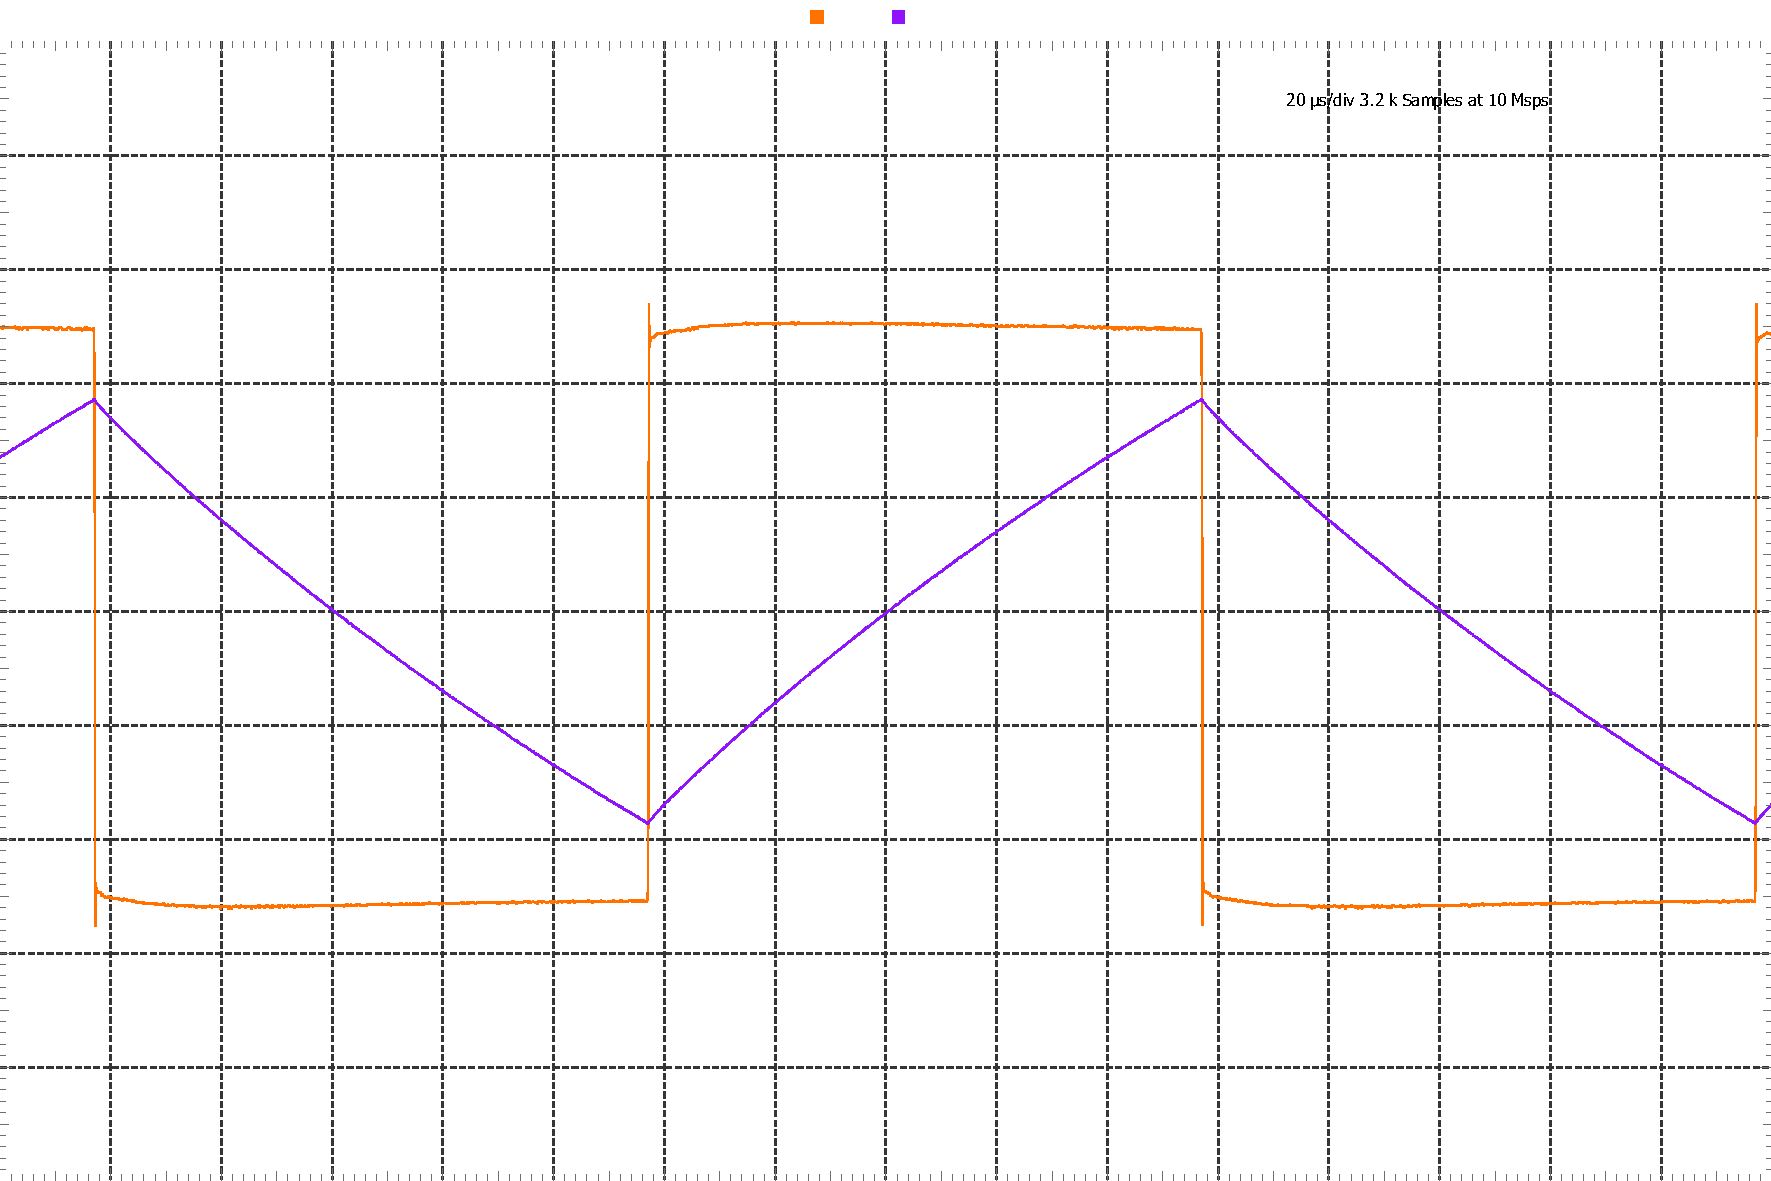
\includegraphics[width=\textwidth]{05_scopy1}
	\caption{Oscilloscope display for Circuit Three}
	\label{fig:circuit3oscope}
\end{figure}

Notice how the purple waveform gets nearly to the top level of the input
waveform. This is the expected outcome.

Comparing this to the SPICE analysis in Figure \ref{fig:circuit3pspice},

\begin{figure}[H]
	\centering
	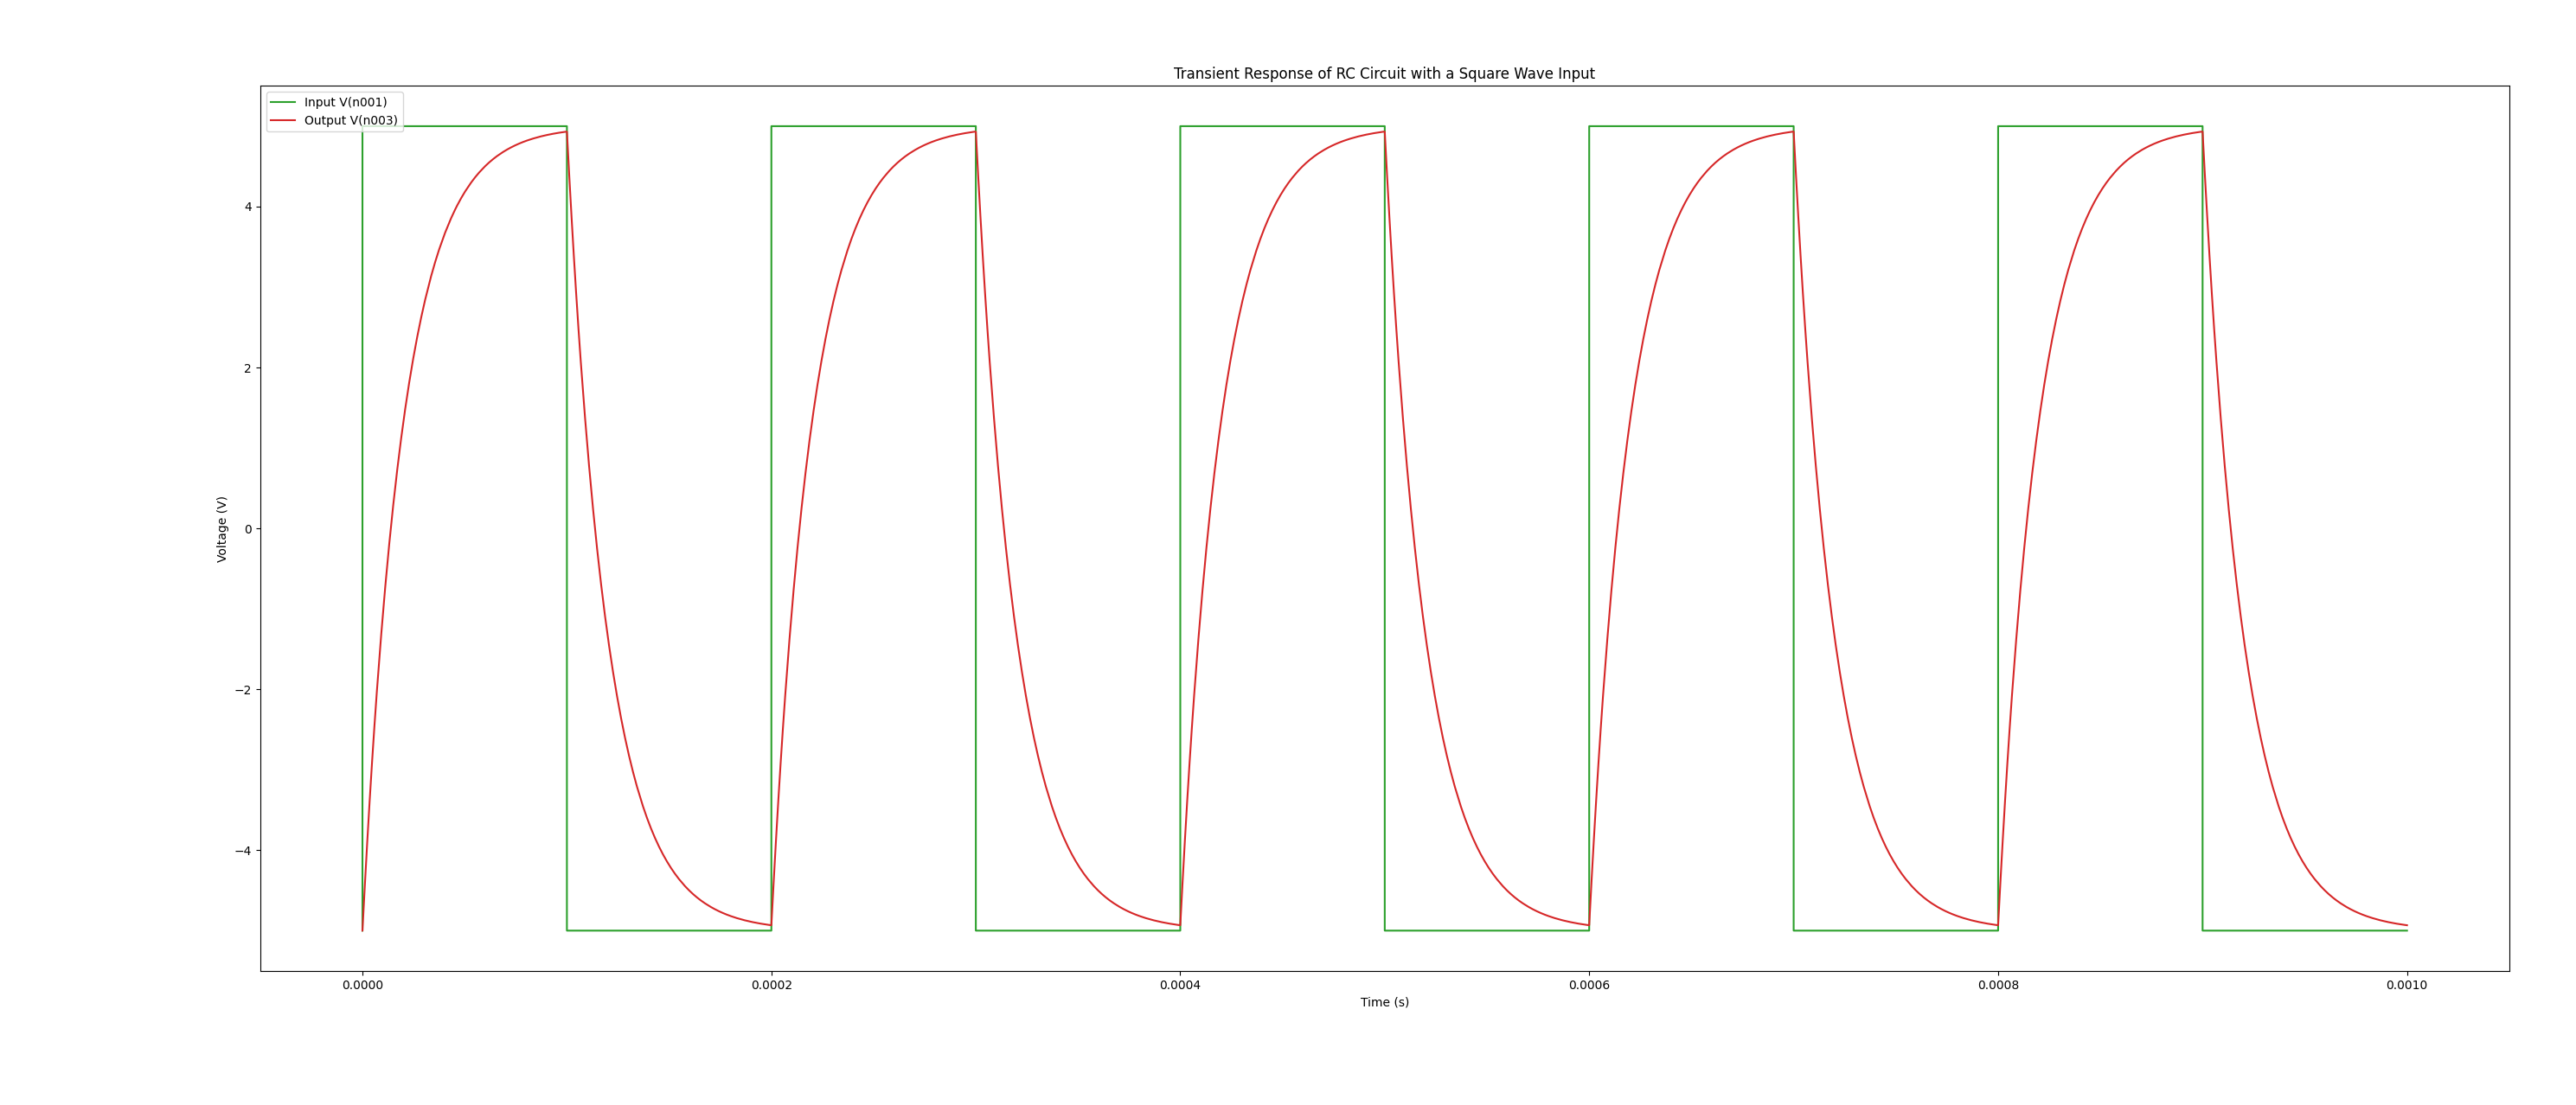
\includegraphics[width=\textwidth]{05_ltspicecircuit3}
	\caption{LTSpice Simulated Values}
	\label{fig:circuit3pspice}
\end{figure}

\subsubsection{Analysis}


To determine the experimental time constant, we observe the waveform in Figure \ref{fig:circuit3oscope}. The purple trace, representing the voltage across the capacitor, follows an exponential charging and discharging curve in response to the square wave input.

The signal generator was set to a square wave of frequency $f = 5\,\mathrm{kHz}$, corresponding to a period:
\[
	T = \frac{1}{f} = \frac{1}{5\,000} = 200\,\mu\mathrm{s}
\]

Since the square wave toggles every half period, each high or low duration is:
\[
	T_{\text{high}} = T_{\text{low}} = \frac{T}{2} = 100\,\mu\mathrm{s}
\]

Our calculated time constant was $\tau = 20\,\mu\mathrm{s}$, meaning:
\[
	\frac{T_{\text{high}}}{\tau} = \frac{100\,\mu\mathrm{s}}{20\,\mu\mathrm{s}} = 5
\]

This matches the rule of thumb that a capacitor reaches over 99\% of its final value after 5 time constants. The purple waveform nearly reaches the full amplitude of the orange square wave before discharging again, consistent with this theoretical behavior.

Comparing this to the LTSpice simulation in Figure \ref{fig:circuit3pspice}, we
observe excellent agreement. Both the simulated and measured waveforms exhibit
the same exponential rise and fall within the $100\mu s$ half-period.

Therefore, the experimental time constant agrees well with both the calculated value and the simulated output, with only minimal deviation due to real-world component tolerances and scope sampling resolution.
\subsection{Circuit Four: Square Wave Response}

Circuit four had a frequency calculated for its input square wave of $10\,\mathrm{kHz}$ due
to the change in the sizes of both the resistive and capacitive portions of the
circuit. This higher frequency results in a shorter available charge/discharge window per cycle.

\begin{figure}[H]
	\centering
	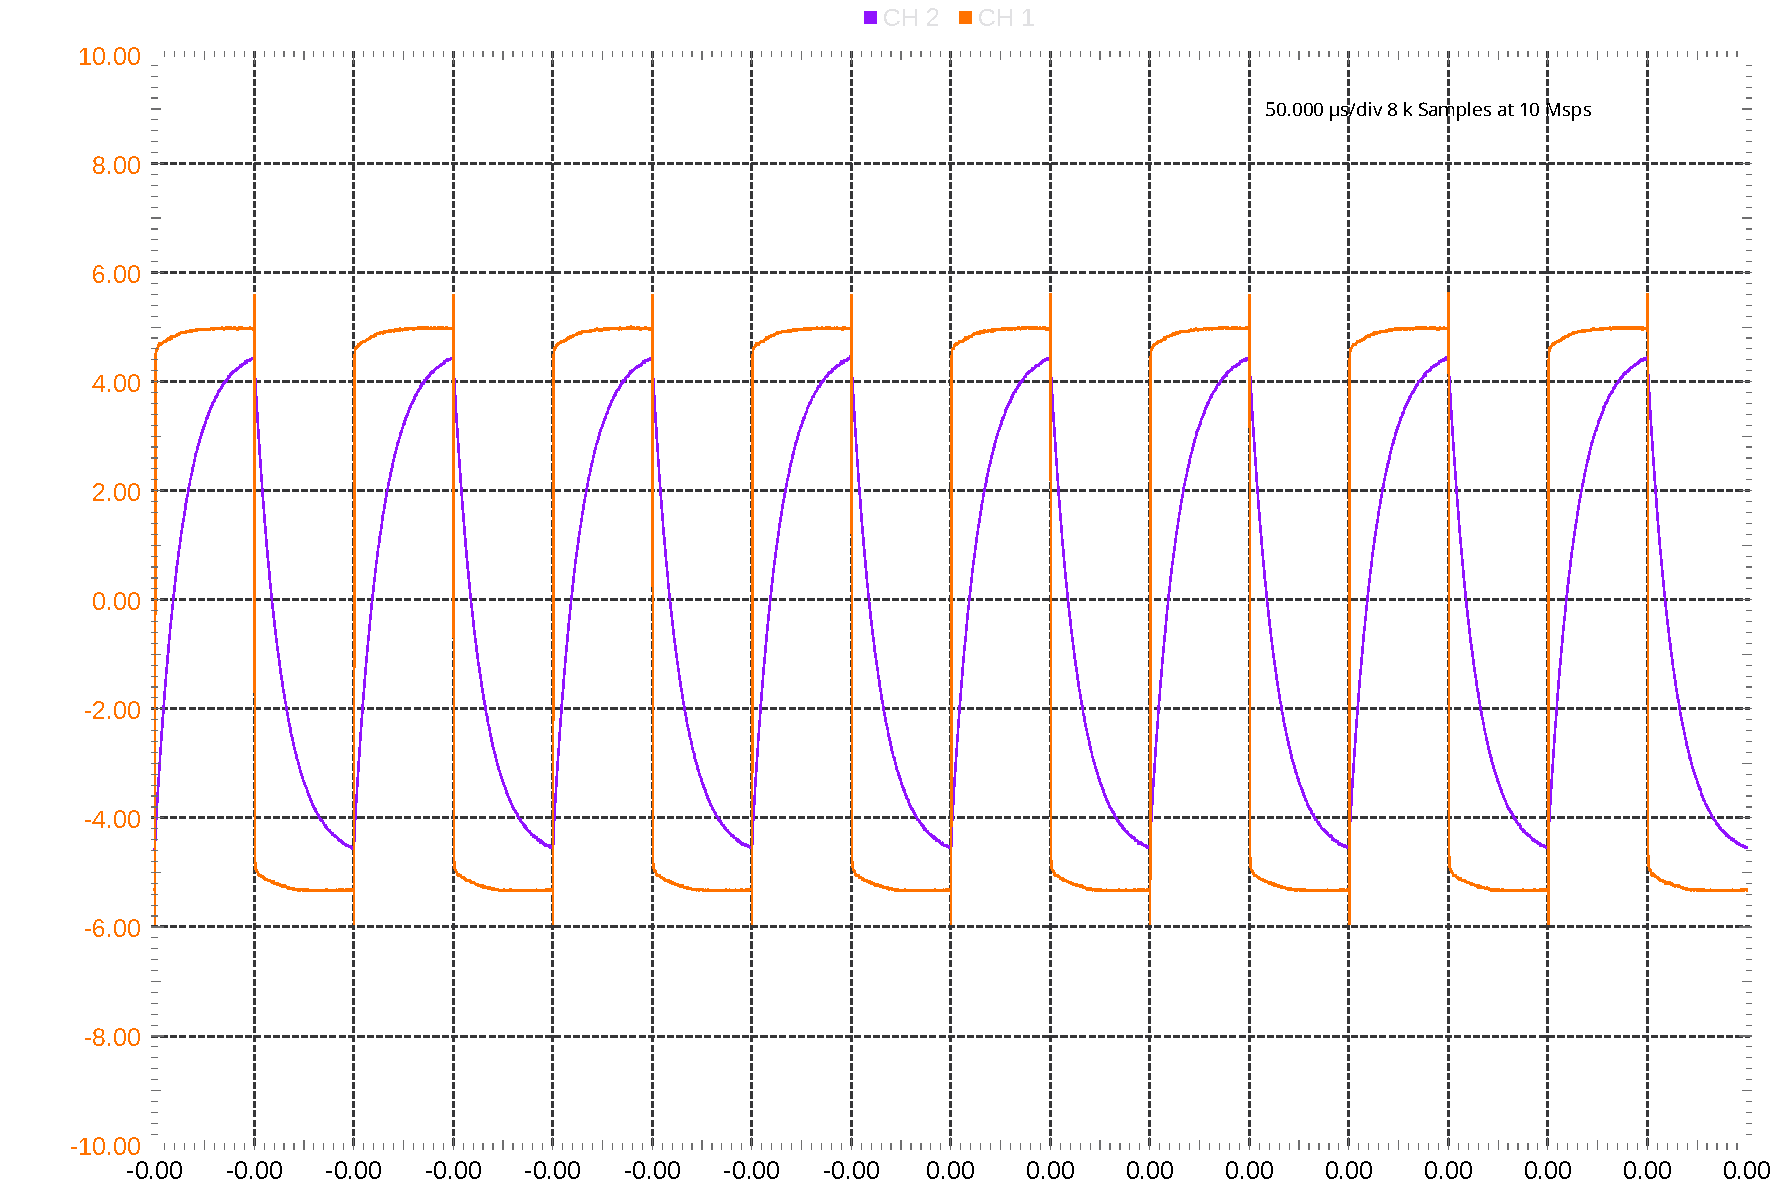
\includegraphics[width=16cm]{05_scopy2}
	\caption{Oscilloscope display for Circuit Four}
	\label{fig:circuit4oscope}
\end{figure}

\subsubsection{Analysis}
The signal generator was set to a $10\,\mathrm{kHz}$ square wave, giving a full period of:
\[
	T = \frac{1}{f} = \frac{1}{10\,000} = 100\,\mu\mathrm{s}
\]
With the square wave toggling every half-cycle:
\[
	T_{\text{high}} = T_{\text{low}} = 50\,\mu\mathrm{s}
\]

The time scale in Figure \ref{fig:circuit4oscope} confirms that the capacitor
does not fully charge or discharge before the square wave switches direction,
which is expected. The waveform (purple) rises and falls exponentially, but does
not reach the full $5V$ input level due to the shorter available time. This matches the calculated design for a smaller time constant relative to Circuit Three.

From the image, the capacitor reaches approximately 63\% of its full excursion within one-fifth of the half-period, suggesting:
\[
	\tau_{\text{exp}} \approx \frac{50\,\mu\mathrm{s}}{5} = 10\,\mu\mathrm{s}
\]

This agrees with the calculated value used to determine the input frequency. The exponential curves and timing visually confirm this result.

\subsubsection{SPICE Simulation}

Comparing this to the LTSpice simulation in Figure \ref{fig:circuit4pspice}, the agreement is excellent. The red curve (capacitor voltage) in simulation matches the real purple waveform in both shape and amplitude behavior, undershooting the full square wave level due to insufficient time per cycle to reach steady-state.

\begin{figure}[H]
	\centering
	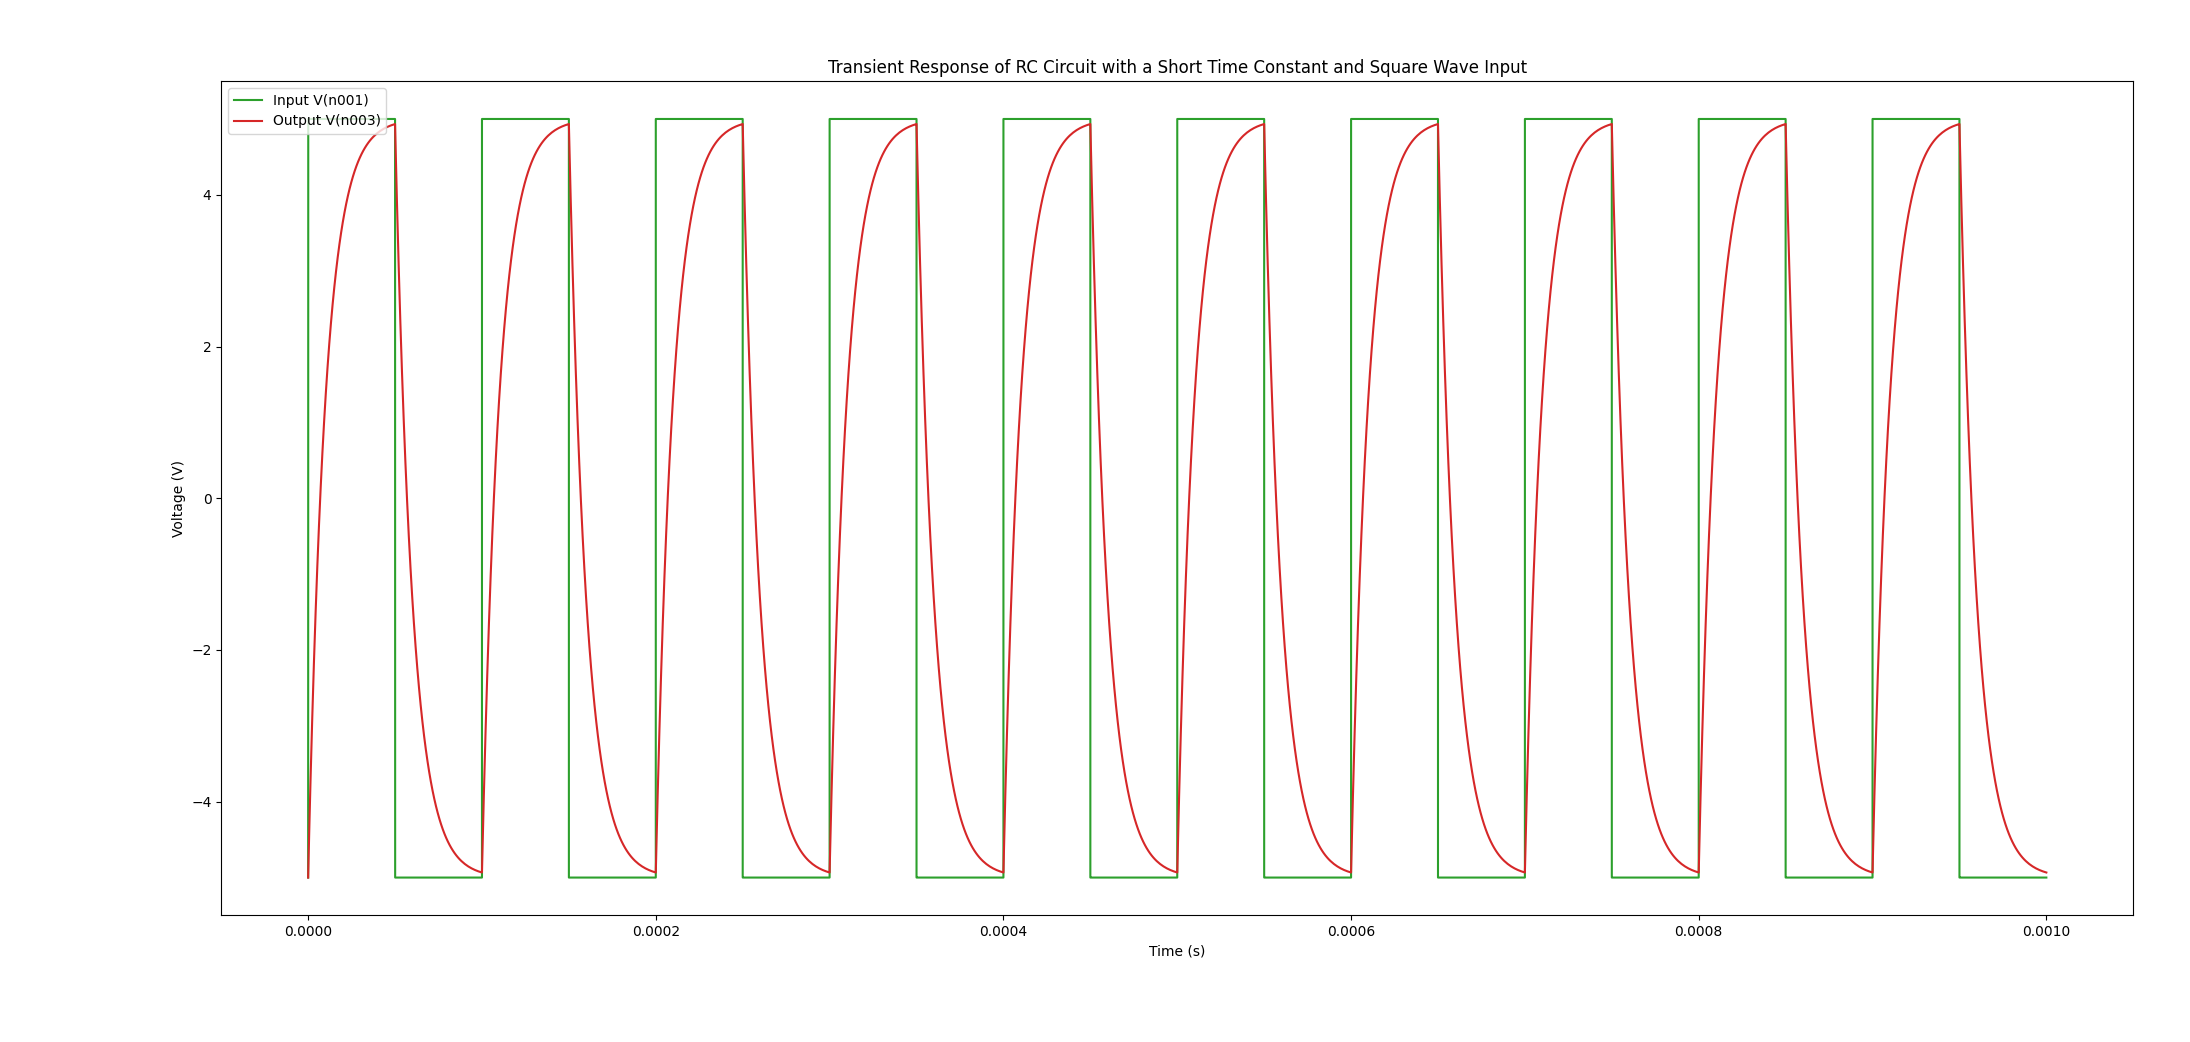
\includegraphics[width=16cm]{05_ltspicecircuit4}
	\caption{LTSpice Simulated Values}
	\label{fig:circuit4pspice}
\end{figure}

The experimental data strongly agrees with both the theoretical time constant and the LTSpice simulation. The waveform exhibits behavior exactly predicted by the time constant formula, and the result confirms the exponential nature of the charging and discharging phases even in rapid time-domain switching scenarios.
\subsection{Circuit Five: RL Circuit Response}

Utilizing a smaller amplitude of $1\,\mathrm{V}$ and a frequency of $1\,\mathrm{kHz}$, the following waveform was output from the implemented RL circuit. This circuit replaces the capacitive element with an inductive one, introducing a fundamentally different dynamic governed by the inductor’s opposition to changes in current.

\begin{figure}[H]
	\centering
	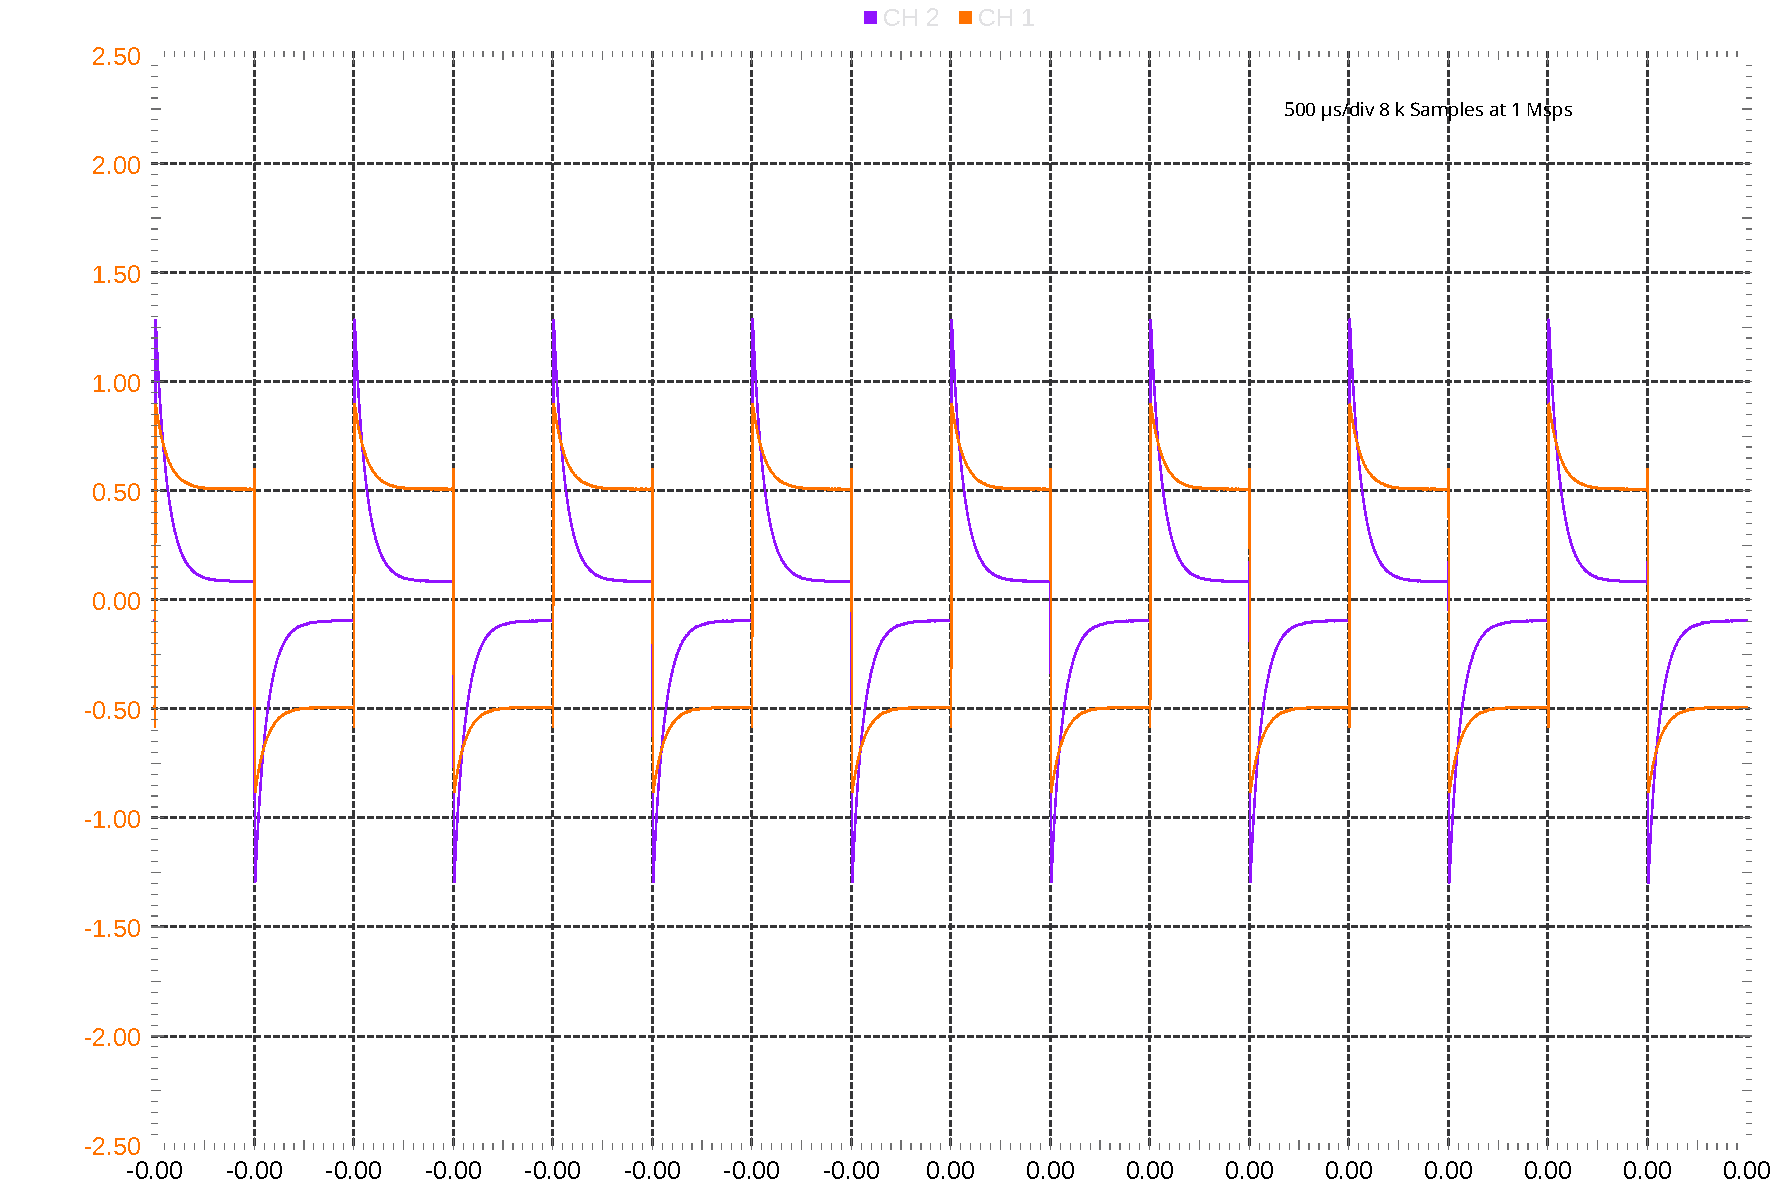
\includegraphics[width=16cm]{05_scopy3}
	\caption{Oscilloscope display for Circuit Five}
	\label{fig:circuit5oscope}
\end{figure}

\subsubsection{Analysis}
In contrast to RC circuits, the voltage waveform here displays characteristic spikes at each edge of the square wave. These voltage discontinuities occur because an inductor resists sudden changes in current, not voltage. At the exact moment of a step input (rising or falling), the current through the inductor cannot jump instantaneously, so the voltage must spike to force the change in current.

The waveform captured in Figure \ref{fig:circuit5oscope} shows these expected traits clearly. The orange trace is the square wave input (channel 1), while the purple trace (channel 2) shows the voltage across the inductor. As the square wave toggles, the inductor generates a back-emf that causes a voltage spike opposite the direction of the step, then decays exponentially as the current ramps up or down.

Given the input frequency of $1\,\mathrm{kHz}$, the period is:
\[
	T = \frac{1}{f} = 1\,\mathrm{ms}
	\quad \Rightarrow \quad
	T_{\text{high}} = T_{\text{low}} = 0.5\,\mathrm{ms}
\]

The observed time it takes for the purple trace to decay to near zero aligns with an exponential curve over one or two time constants. This supports the theoretical result that:
\[
	\tau = \frac{L}{R}
\]
where $\tau$ is small enough that the system settles during each half-period.

\subsubsection{SPICE Simulation}

\begin{figure}[H]
	\centering
	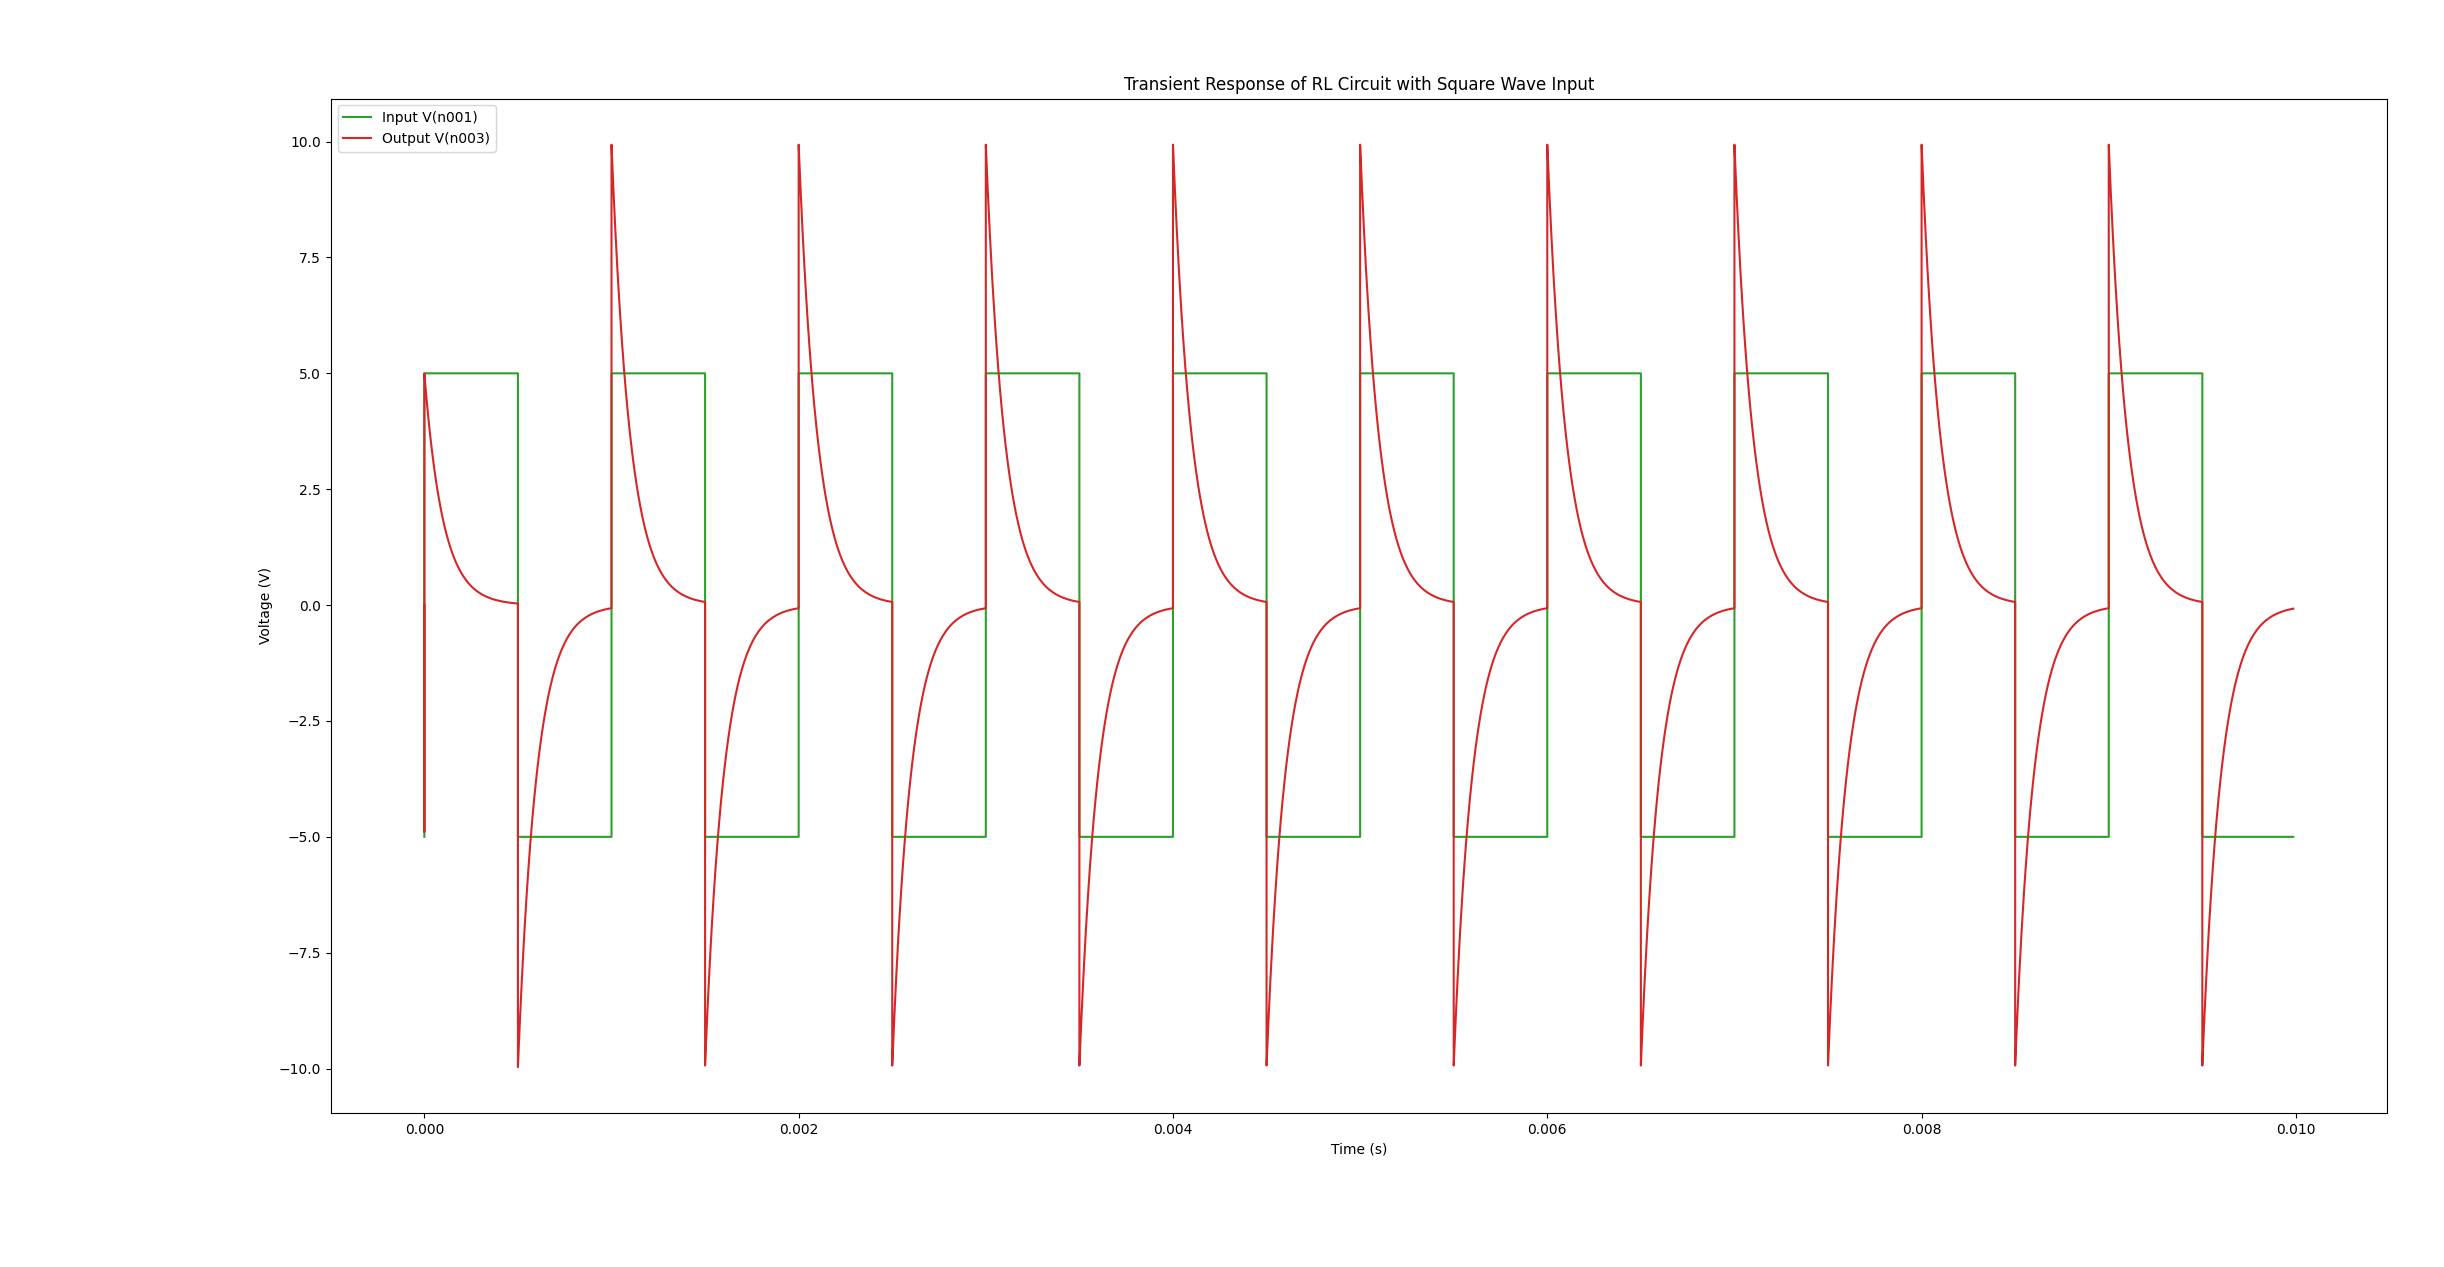
\includegraphics[width=16cm]{05_ltspicecircuit5}
	\caption{SPICE Simulated Values}
	\label{fig:circuit5pspice}
\end{figure}

Figure \ref{fig:circuit5pspice} shows the simulated waveform for the same RL configuration. Here, the red trace (inductor voltage) spikes at each transition and then decays exponentially, matching both the measured waveform and theoretical expectations. The simulation shows these transitions more cleanly because it doesn’t account for practical limitations like inductor non-idealities or noise.

The experimental RL waveform exhibits behavior expected of an inductor-dominant circuit. The voltage across the inductor spikes when the square wave toggles and then decays, in accordance with $\tau = \frac{L}{R}$. Both the oscilloscope data and the LTSpice simulation agree, confirming the transient behavior of inductors under periodic forcing functions.
\section{Conclusion}

This lab served to introduce and explore the concept of first-order circuits—those containing either capacitors or inductors alongside resistors—and demonstrated their distinctive exponential behaviors through both long and short time constant scenarios. 

From the slow voltage ramp in the high-impedance RC circuit to the rapid switching transients in the square wave experiments, the exponential form governed each response consistently. The experimental work reinforced the theory: capacitors resist changes in voltage and settle over time as they charge or discharge, while inductors oppose changes in current, generating voltage spikes as they adjust to new current levels.

SPICE simulations matched the measured results across all configurations, confirming both the validity of the exponential time constant model and the effect of real-world tolerances. Discrepancies in the RC measurements—such as reduced final voltages—highlighted the importance of accounting for the input resistance of test equipment when working with high-impedance circuits.

Ultimately, by understanding the role of $\tau$ in shaping transient behavior, the analysis of first-order circuits becomes intuitive and efficient—requiring only a few well-chosen constants and a solid grasp of exponential dynamics to fully characterize a circuit's response over time.
\end{document}
% vim: set ft=tex tw=80 ts=2 sts=2 sw=2 noet spell:
